% ============================================================
%  Double Descent Report — LaTeX Source
%  Empirical Reproduction of Double Descent in Linear Regression
% ============================================================
\documentclass[12pt, a4paper]{article}

% ── Core packages ──────────────────────────────────────────
\usepackage[a4paper, top=2.5cm, bottom=2.5cm, left=2.8cm, right=2.8cm]{geometry}
\usepackage[utf8]{inputenc}
\usepackage[T1]{fontenc}
\usepackage[activate={true,nocompatibility},tracking=true,kerning=true,spacing=false,factor=1100,stretch=0,shrink=0]{microtype}

% ── Mathematics ────────────────────────────────────────────
\usepackage{amsmath}
\usepackage{amssymb}
\usepackage{mathtools}
\usepackage{bm}

% ── Figures & Tables ───────────────────────────────────────
\usepackage{graphicx}
\usepackage{booktabs}
\usepackage{array}
\usepackage{float}
\usepackage{caption}
\usepackage{subcaption}
\captionsetup{font=small, labelfont=bf, margin=10pt}

% ── Colours & hyperlinks ───────────────────────────────────
\usepackage[dvipsnames]{xcolor}
\definecolor{accentblue}{RGB}{31, 78, 121}
\definecolor{lightgray}{RGB}{245, 245, 245}
\definecolor{darkgray}{RGB}{80, 80, 80}
\usepackage[
  colorlinks = true,
  linkcolor  = black,
  citecolor  = accentblue,
  urlcolor   = accentblue,
  pdftitle   = {Double Descent Report},
  pdfauthor  = {},
  bookmarks  = true,
  bookmarksopen = false
]{hyperref}

% ── Section styling ────────────────────────────────────────
\usepackage{titlesec}
\titleformat{\section}
  {\large\bfseries}{\thesection.}{0.6em}{}[\vspace{-2pt}\vspace{2pt}]
\titleformat{\subsection}
  {\normalsize\bfseries}{\thesubsection}{0.5em}{}
\titleformat{\subsubsection}
  {\normalsize\bfseries}{\thesubsubsection}{0.5em}{}
\titlespacing*{\section}{0pt}{14pt}{6pt}
\titlespacing*{\subsection}{0pt}{10pt}{4pt}


% ── List & spacing ─────────────────────────────────────────
\usepackage{enumitem}
\setlist[itemize]{leftmargin=*, topsep=3pt, itemsep=2pt}
\setlist[enumerate]{leftmargin=*, topsep=3pt, itemsep=2pt}
\usepackage{parskip}
\setlength{\parskip}{6pt}
\setlength{\parindent}{0pt}

% ── Bibliography ───────────────────────────────────────────
\usepackage[numbers, sort&compress]{natbib}
\bibliographystyle{unsrtnat}

% ── Utility ────────────────────────────────────────────────
\usepackage{mdframed}
\newmdenv[
  backgroundcolor = lightgray,
  linecolor       = black,
  linewidth       = 1pt,
  leftmargin      = 0pt,
  rightmargin     = 0pt,
  innerleftmargin = 10pt,
  innerrightmargin= 10pt,
  innertopmargin  = 8pt,
  innerbottommargin=8pt,
  skipabove       = 8pt,
  skipbelow       = 8pt
]{keybox}

% ── Convenience macros ─────────────────────────────────────
\newcommand{\R}{\mathbb{R}}
\newcommand{\E}{\mathbb{E}}
\newcommand{\norm}[1]{\left\lVert #1 \right\rVert}
\newcommand{\pinv}{X^{+}}

% ============================================================
\begin{document}
% ============================================================

% ── Title page ─────────────────────────────────────────────
\begin{titlepage}
  \newgeometry{left=3cm, right=3cm, top=3cm, bottom=3cm}
  \centering


\includegraphics[width=0.3\textwidth]{logo.png}\\[0.8cm]

  {\LARGE\bfseries

  \textbf{Double Descent in Linear Models}
  }

  \vspace{4cm}

  {\huge\bfseries Mahyar MohammadiMatin}\\[0.5cm]
  {\large Student Number: 53350A}\\[2cm]

  {\small\color{darkgray}
  I declare that this material, which I now submit for assessment, is entirely my own work and has not been taken from
  the work of others, save and to the extent that such work has been cited and acknowledged within the text of my work.
  I understand that plagiarism, collusion, and copying are grave and serious offences in the university and accept the
  penalties that would be imposed should I engage in plagiarism, collusion or copying. This assignment, or any part of it,
    has not been previously submitted by me or any other person for assessment on this or any other course of study.
  }
\vfill
  {\large Machine Learning Course Experimental Project}\\[0.3cm]
  {June 2026}



  {\rule{\linewidth}{1pt}}
  \restoregeometry
\end{titlepage}

\thispagestyle{empty}
\tableofcontents
\newpage

% ============================================================
\section{Introduction}
% ============================================================

A central question in supervised machine learning is: how does a model's complexity affect its ability to generalise to unseen data? For decades, the standard answer was the bias-variance trade-off, a well-established theoretical framework that prescribes an optimal intermediate level of model complexity: neither too simple nor too expressive. This principle guided decades of model selection, regularisation design, and the overall philosophy of avoiding over-parameterisation.

Recent empirical work by Belkin et al.~\cite{belkin2019reconciling} (\textit{``Reconciling Modern Machine Learning Practice and the Bias-Variance Trade-off''})has revealed that this picture is fundamentally incomplete. In practice, modern models such as deep neural networks and kernel machines are trained with far more parameters than training samples, yet continue to generalise well. This observation directly contradicts classical theory.

The key insight is that the test-error curve is not U-shaped, but rather exhibits a second descent: after an initial region of classical behaviour, error spikes catastrophically at the interpolation threshold (where the model exactly fits the training data), and then surprisingly continues to decrease as the model becomes even more over-parameterised.

This project empirically reproduces the double descent phenomenon in the well-controlled setting of linear regression, using a synthetic dataset with noisy linear labels. Three learning methods are implemented entirely from scratch:

1.Ordinary Least Squares,
2.Ridge Regression,
3.Gradient Descent

By systematically varying the model's dimensionality $d$ while fixing the number of training points $n$, we trace the full double descent curve, identify the interpolation threshold at $d = n$, and analyse how regularisation (both explicit and implicit) tames the catastrophic failure near that threshold.

% ============================================================
\section{Background Theory}
% ============================================================

\subsection{Classical Bias-Variance Trade-off}

In classical statistical learning theory, the expected test error of any estimator $\hat{f}$ can be decomposed as:

\begin{equation}
  \E\!\left[(y - \hat{f}(x))^2\right]
  \;=\;
  \underbrace{\mathrm{Bias}^2(\hat{f})}_{\text{systematic error}}
  +\;
  \underbrace{\mathrm{Var}(\hat{f})}_{\text{sensitivity to data}}
  +\;
  \underbrace{\sigma^2}_{\text{irreducible noise}}
  \label{eq:bv}
\end{equation}

The framework predicts a characteristic U-shaped test-error curve: as complexity increases, bias decreases while variance increases, and the optimal model lies at the trough somewhere in an intermediate complexity region. This advises practitioners to avoid both under-parameterised models (high bias) and over-parameterised models (high variance), and to use regularisation to find the sweet spot.

This classical picture breaks down in modern high-capacity models. Deep neural networks (which routinely operate with millions of parameters trained on thousands of examples) generalise remarkably well despite extreme over-parameterisation.

\subsection{The Double Descent Phenomenon}

The double descent curve describes the full behaviour of test error across the entire spectrum of model complexity:

\begin{enumerate}
  \item \textbf{Classical scenario} ($d \ll n$): The OLS problem has a \textbf{unique solution} but the model cannot interpolate the training data. Test error follows the classical U-shape: initially high (underfitting), then decreasing as complexity grows.
  \item \textbf{Interpolation threshold} ($d \approx n$): $X$ is square. The model has just enough parameters to perfectly fit the training data. The solution is highly unstable and numerically ill-conditioned. Test error spikes to its global maximum.
  \item \textbf{Modern over-parameterised scenario} ($d \gg n$): Many solutions interpolate the training data. Among these, the \textbf{minimum-norm solution} (selected by the pseudoinverse) turns out to generalise well. Test error descends again, often below the classical minimum.
\end{enumerate}

The intuition for the third phase is that as $d$ grows, the model has ever more freedom in weight space. The minimum-norm interpolant becomes increasingly smooth and naturally regularised as the ambient dimension increases.

% ============================================================
\section{Mathematical Foundations}
% ============================================================

\subsection{Data Generation}

We generate a synthetic regression dataset where the true relationship is linear with added Gaussian noise. Given $n$ total samples in $d$ dimensions:
\[
  X \in \R^{n \times d},\quad X_{ij} \overset{\text{i.i.d.}}{\sim} \mathcal{N}(0,1)
\]
The true weight vector is drawn as:
\[
  w^* \in \R^d,\quad w^*_j \sim \mathcal{N}\!\left(0,\,\tfrac{1}{d}\right)
\]
Scaling by $1/\sqrt{d}$ keeps the expected signal magnitude $\norm{Xw^*}$ roughly stable as $d$ varies, ensuring a fair comparison across dimensions. The noisy targets are:
\begin{equation}
  y = Xw^* + \varepsilon, \qquad \varepsilon \sim \mathcal{N}(0, \sigma^2 I)
  \label{eq:dgp}
\end{equation}

\subsection{Ordinary Least Squares}

Ordinary Least Squares (OLS) minimises the squared residual ${L}(w) = \norm{Xw - y}_2^2$.

\subsubsection*{Overdetermined case ($d < n$)}
When $X^TX$ is invertible (full column rank), the unique solution is:
\begin{equation}
  \hat{w}_{\mathrm{OLS}} = (X^TX)^{-1}X^Ty
  \label{eq:ols}
\end{equation}

\subsubsection*{Underdetermined case ($d > n$)}
The system $Xw = y$ has infinitely many solutions. The \textbf{minimum-norm least-squares solution} is obtained via the Moore-Penrose pseudoinverse $X^+ = X^T(XX^T)^{-1}$:
\begin{equation}
  \hat{w}_{\mathrm{min\text{-}norm}} = X^+y = X^T(XX^T)^{-1}y
  \label{eq:minnorm}
\end{equation}

For the case that $XX^T$ is not invertible, if we have $X = U\Sigma V^T$ (SVD) then:
\begin{equation}
  X^+ = V\Sigma^+U^T
  \label{eq:svd_pinv}
\end{equation}
This is the unique solution to $\min_w \norm{w}_2^2$ subject to $Xw = y$.

\subsection{Ridge Regression}

Ridge regression adds an $\ell_2$ penalty on the weight norm:
\begin{equation}
  \mathcal{L}_\lambda(w) = \norm{Xw - y}_2^2 + \lambda\norm{w}_2^2, \qquad \lambda > 0
  \label{eq:ridge_loss}
\end{equation}
Setting $\nabla_w \mathcal{L}_\lambda = 0$:
\[
  2X^T(Xw - y) + 2\lambda w = 0 \quad\Longrightarrow\quad (X^TX + \lambda I)\,w = X^Ty
\]
The unique solution is:
\begin{equation}
  \hat{w}_{\mathrm{ridge}} = (X^TX + \lambda I)^{-1}X^Ty
  \label{eq:ridge}
\end{equation}
The matrix $X^TX + \lambda I$ is \textbf{always invertible} for $\lambda > 0$, regardless of whether $X$ is rank-deficient, because $\lambda I$ shifts all eigenvalues of $X^TX$ by $+\lambda$, replacing any zero eigenvalues with $\lambda > 0$.

\subsection{Gradient Descent on the Least Squares Objective}

Gradient descent iteratively updates the weight vector:
\begin{equation}
  w^{(t+1)} = w^{(t)} - \eta\,\nabla_w\mathcal{L}(w^{(t)})
  \label{eq:gd_update}
\end{equation}
For the OLS objective $\mathcal{L}(w) = \norm{Xw - y}_2^2$, the gradient is $\nabla_w\mathcal{L}(w) = 2X^T(Xw - y)$, giving:
\begin{equation}
  w^{(t+1)} = w^{(t)} - \frac{2\eta}{n}\,X^T(Xw^{(t)} - y)
  \label{eq:gd}
\end{equation}
where $\eta > 0$ is the learning rate and $w^{(0)} = {0}$.

\textbf{Implicit regularisation of GD.} As $T \to \infty$, it converges to the \emph{minimum-norm} solution $\hat{w}_{\mathrm{min\text{-}norm}}$, not an arbitrary interpolant. For finite $T$, the iterates are equivalent to a ridge estimator with implicit regularisation strength that \emph{decreases} as $T$ increases:
\[
  \text{Few iterations} \;\longleftrightarrow\; \text{Large effective }\lambda \;\longleftrightarrow\; \text{Strong regularisation}
\]

\subsection{Model Complexity and the Condition Number}

The \textbf{condition number} of the training matrix $X_{\mathrm{train}}$ is defined as:
\begin{equation}
  \kappa(X) = \frac{\sigma_{\max}(X)}{\sigma_{\min}(X)}
  \label{eq:cond}
\end{equation}
where $\sigma_{\max}$ and $\sigma_{\min}$ are the largest and smallest singular values, respectively.
$\kappa$ refers to how much the output (solution) of a calculation can change when the input (data) has small errors or changes.

\begin{itemize}
  \item $\kappa \approx 1$: Well-conditioned; An error in the input is not amplified at all.
  \item $\kappa$ is very large (e.g., 1,000, 1 million) : Ill-conditioned; small perturbations in $y$ produce large changes in $\hat{w}$, catastrophically amplifying noise.
  \item $\kappa \to \infty$: Singular; the matrix is not invertible and OLS has no unique solution.
\end{itemize}

Near $d = n$, the training matrix develops near-zero eigenvalues, causing $\kappa$ to diverge. This is the root cause of the test-error spike at the interpolation threshold.

\subsection{Evaluation: Mean Squared Error}

Models are evaluated with \textbf{Mean Squared Error} {MSE}_{\mathrm{test}}  = \frac{1}{n_{\mathrm{test}}}  \sum_{i=1}^{n_{\mathrm{test}}}  (y_i - \hat{y}_i)^2.

Experiments are averaged over multiple seeds to reduce variance and produce smooth, reliable estimates of expected generalisation error (specially near interpolation).

% ============================================================
\section{Experimental Setup}
% ============================================================

All experiments share the following structure:

\begin{table}[H]
  \centering
  \caption{Global experimental parameters.}
  \label{tab:params}
  \renewcommand{\arraystretch}{1.35}
  \begin{tabular}{
    >{\bfseries}l
    l
  }
    \toprule
    Parameter & Value \\
    \midrule
    Training samples ($n_{\mathrm{train}}$) & 100 \\
    Test samples ($n_{\mathrm{test}}$)       & 1{,}000 \\
    Dimension range ($d$)                    & 10 to 200, step 5 \\
    Noise levels ($\sigma$)                  & 0.2, 0.4, 0.8 \\
    Random seeds                             & 10 seeds, averaged \\
    Interpolation threshold                  & $d = n = 100$ \\
    \bottomrule
  \end{tabular}
\end{table}

% ============================================================
\section{Results and Analysis}
% ============================================================

\subsection{Condition Number Analysis}

\begin{figure}[H]
  \centering
  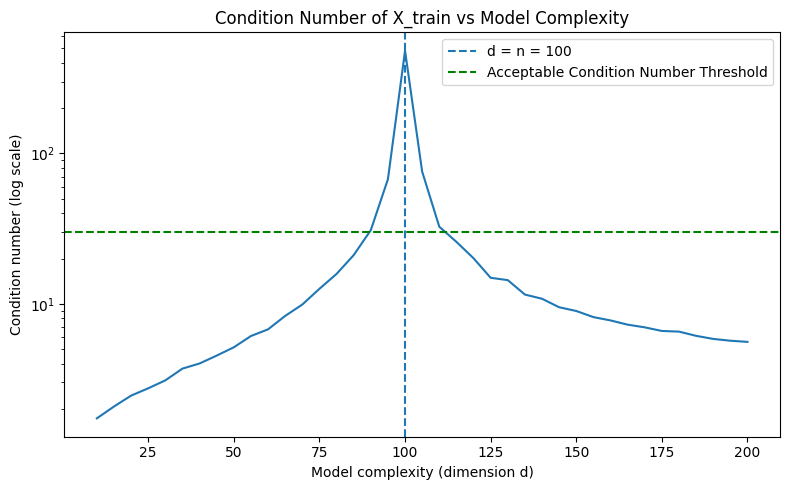
\includegraphics[width=0.72\textwidth]{figure_1.png}
  \caption{Condition number of the training matrix $X_{\mathrm{train}}$ as a function of model dimension $d$ (averaged over seeds, log scale). The dashed blue line marks the interpolation threshold $d = n = 100$; the dashed green line marks an acceptable condition number threshold of 30.}
  \label{fig:cond}
\end{figure}

Figure~\ref{fig:cond} reveals the geometric basis of the double descent phenomenon with striking clarity.

\textbf{Underparameterised scenario} ($d < 100$). The condition number increases gradually and monotonically as $d \to n$. As we add more dimensions, the columns of $X_{\mathrm{train}}$ begin to align more closely, increasing ill-conditioning. Importantly, $\kappa$ remains well below 30 for most of this range, meaning OLS inversions are numerically stable.

\textbf{At the interpolation threshold} ($d = n = 100$). The condition number spikes dramatically to approximately $1000$. This is the critical numerical singularity: $X_{\mathrm{train}}$ is square ($100 \times 100$), and any slight numerical deficiency in its rank causes the matrix to become nearly non-invertible. This will produce an extremely unstable weight vector with enormous norm and catastrophically poor test error.

\textbf{Overparameterised scenario} ($d > 100$). After the spike, the condition number drops and stabilises well below 30 and as $d$ grows, the minimum-norm solution becomes progressively better-behaved.

\begin{keybox}
\textbf{Key Takeaway.} The catastrophic test-error spike at $d = n$ has a direct numerical cause: the condition number of $X_{\mathrm{train}}$ diverges exactly at this point. Regularisation methods (ridge, early stopping) work precisely by bounding this condition number.
\end{keybox}

\subsection{Least Squares: Observing the Double Descent Curve}

\begin{figure}[H]
  \centering
  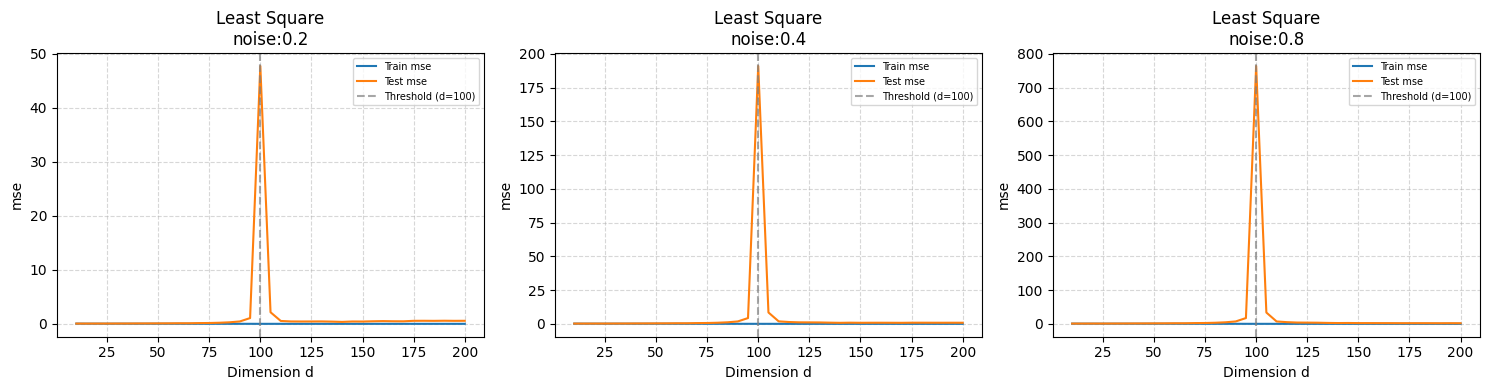
\includegraphics[width=\textwidth]{figure_2.png}
  \caption{Train MSE (blue) and Test MSE (orange) for Ordinary Least Squares across dimensions $d \in [10, 200]$ for three noise levels: $\sigma = 0.2$ (left), $\sigma = 0.4$ (centre), $\sigma = 0.8$ (right). The dashed vertical line marks the interpolation threshold at $d = 100$.}
  \label{fig:ols}
\end{figure}

Figure~\ref{fig:ols} is reproducing the classical double descent curve in its full form.

\textbf{Train error (blue).} The training MSE behaves exactly as predicted by theory. For $d < n$, training error is non-zero, the model lacks the degrees of freedom to interpolate. For $d \geq n$, training error drops to effectively zero for \emph{all} noise levels. This is the definition of interpolation: the model memorises every training point perfectly, including the noise.

\textbf{Test error (orange).} This is where the double descent phenomenon lives:
\begin{enumerate}
  \item \textbf{Classical descent} ($d \ll n$, roughly $d < 70$): Test error starts moderate and slowly decreases as the model gains capacity to learn the true signal. This is the classical "bias reduction" part of the U-shape.
  \item \textbf{Pre-threshold increase} ($70 < d < 100$): As $d \to n$, test error rises and complexity accumulates faster than the data can control it. This is the classical "variance increase" that forms the right arm of the U.
  \item \textbf{Catastrophic spike at} $d = n$: Test error explodes at the interpolation threshold. The magnitude scales strongly with noise. This scaling reflects the condition-number amplification of noise.
  \item \textbf{Second descent} ($d > n$): After the spike, test error falls dramatically. As $d$ grows beyond 100, the minimum-norm interpolant becomes progressively better-regularised and test error decreases.
\end{enumerate}

The qualitative shape is identical across all three noise levels, confirming that double descent is a robust phenomenon rather than a low-noise artefact.

\subsection{Ridge Regression}

\begin{figure}[H]
  \centering
  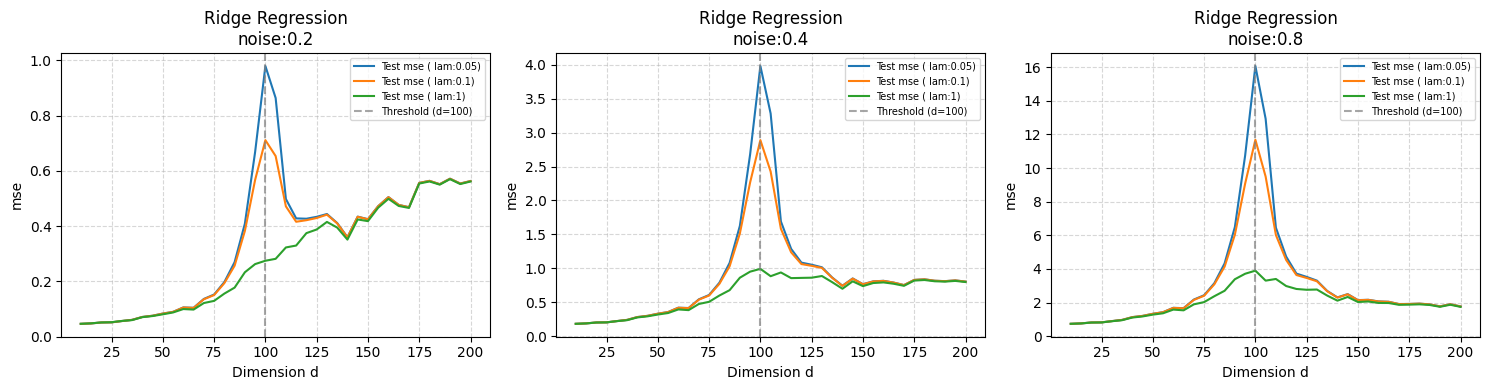
\includegraphics[width=\textwidth]{figure_3.png}
  \caption{Ridge Regression MSE with 3 regularisation strengths ($\lambda \in \{0.05, 0.1, 1\}$) in dimensions $d \in [10, 200]$, for $\sigma = 0.2$ (left), $\sigma = 0.4$ (centre), $\sigma = 0.8$ (right).}
  \label{fig:ridge}
\end{figure}

Figure~\ref{fig:ridge} illustrates how explicit regularisation controls the double descent.

\textbf{Dramatic peak reduction.} Comparing Figure~\ref{fig:ridge} to Figure~\ref{fig:ols}, the spike at $d = n = 100$ is dramatically reduced across all noise levels, even for the weakest regularisation. The mechanism is clear from Equation~\eqref{eq:ridge}: ridge adds $\lambda I$ to $X^TX$, replacing near-zero eigenvalues with $\lambda > 0$ and bounding the effective condition number.

\textbf{Effect of $\lambda$ on curve shape.}
\begin{itemize}
  \item \textbf{Weak regularisation} ($\lambda = 0.05$, blue): The curve closely resembles OLS with a reduced peak. The double descent shape is still visible.
  \item \textbf{Moderate regularisation} ($\lambda = 0.1$, orange): The peak is further reduced, providing a good bias-variance balance.
  \item \textbf{Strong regularisation} ($\lambda = 1$, green): The interpolation peak is almost entirely eliminated.
\end{itemize}

\subsection{Gradient Descent: Implicit Regularisation via Early Stopping}

\begin{figure}[H]
  \centering
  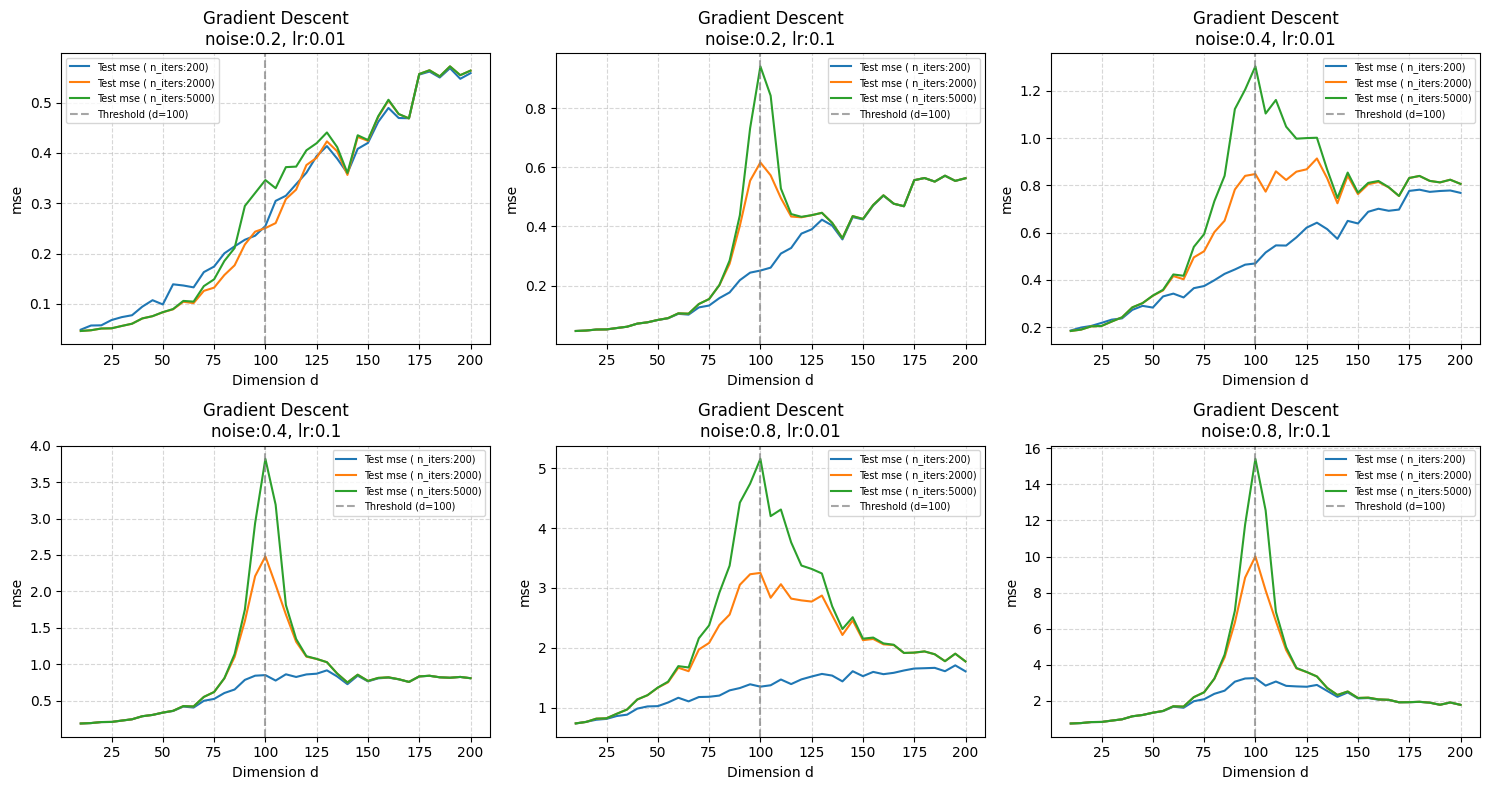
\includegraphics[width=0.85\textwidth]{figure_4.png}
  \caption{Test MSE for Gradient Descent with learning rates $\eta \in \{0.01, 0.1\}$ and iteration counts $T \in \{200, 2000, 5000\}$.}
  \label{fig:gd}
\end{figure}

Figure~\ref{fig:gd} reveals one of the most elegant phenomena in modern machine learning: Fewer iterations = stronger implicit regularisation.
Across both learning rate settings, models trained with fewer iterations ($T = 200$, blue) consistently achieve lower test MSE than those trained for more iterations ($T = 5000$, green), especially near and beyond the interpolation threshold.

\textbf{Effect of learning rate.}
\begin{itemize}
  \item With $\eta = 0.01$: Even 5{,}000 iterations are insufficient for full convergence, so all three curves show significant implicit regularisation. The spread between $T = 200$ and $T = 5{,}000$ is smaller because GD moves slowly and is far from convergence.
  \item With $\eta = 0.1$: Convergence is faster. The $T = 5{,}000$, $\eta = 0.1$ curve is closest to the true OLS/min-norm solution---the peak at $d = 100$ is sharper and more prominent, approximating the OLS behaviour of Figure~\ref{fig:ols}.
\end{itemize}

\textbf{Double descent in GD.} For the highest-convergence setting ($T = 5{,}000$, $\eta = 0.1$, green), the characteristic double descent peak at $d = 100$ is clearly visible, confirming that sufficiently converged GD recovers the same OLS solution and therefore the same double descent behaviour.

\begin{keybox}
\textbf{Practical Implication.} Early stopping is a widely used technique in deep learning, often justified heuristically. These results provide a rigorous explanation: early stopping in gradient descent acts as $\ell_2$ regularisation, and choosing the stopping point is precisely equivalent to tuning $\lambda$ in ridge regression.
\end{keybox}

% ============================================================
\section{Connections to Deep Learning}

Although this study uses simple linear regression, its conclusions extend qualitatively to deep neural networks:

\begin{itemize}
  \item \textbf{Modern deep networks are highly over-parameterised} and trained to near-zero training loss (perfect interpolation), yet generalise well, exactly the behaviour of OLS in the second-descent scenario.
  \item \textbf{SGD with early stopping} is standard practice in deep learning. This work provides an analytical justification: it induces implicit $\ell_2$ regularisation, preventing convergence to the catastrophic interpolation threshold behaviour.
  \item \textbf{Double descent has been observed empirically} in neural networks, kernel machines, and decision tree ensembles~\cite{belkin2019reconciling, nakkiran2020deep}, confirming that the linear regression setting captures the essential mechanism.
\end{itemize}

% ============================================================
\section{Conclusion}
% ============================================================

This project empirically reproduced the \textbf{double descent phenomenon} in linear regression, providing a rigorous and interpretable demonstration that challenges the classical bias-variance trade-off framework. The key findings are:

\begin{enumerate}
  \item \textbf{Classical theory is incomplete.} The test-error curve is not U-shaped but exhibits a second descent after the interpolation threshold at $d = n$.

  \item \textbf{The interpolation threshold is a numerical singularity.} The condition number of $X_{\mathrm{train}}$ peaks sharply at $d = n$, explaining the catastrophic test-error spike. The transition from overdetermined to underdetermined systems passes through a zone of extreme ill-conditioning.

  \item \textbf{Ridge regression weaken the interpolation peak.} By adding $\lambda I$ to $X^TX$, ridge regression bounds the condition number and dramatically reduces the peak.

  \item \textbf{Gradient descent provides implicit regularisation.} GD initialised at zero converges to the minimum-norm solution. With early stopping, it produces solutions equivalent to ridge regression with implicit strength $\propto 1/T$.

  \item \textbf{Noise amplifies all effects.} Higher noise increases the peak at the interpolation threshold proportionally to $\sigma^2$, making regularisation increasingly critical in high-noise settings.
\end{enumerate}

% ============================================================
%  Bibliography
% ============================================================
\begin{thebibliography}{9}

\bibitem{belkin2019reconciling}
M.~Belkin, D.~Hsu, S.~Ma, and S.~Mandal,
``Reconciling modern machine learning practice and the bias-variance trade-off,''
\textit{Proceedings of the National Academy of Sciences},
vol.~116, no.~32, pp.~15849--15854, 2019.

\bibitem{nakkiran2020deep}
P.~Nakkiran, G.~Kaplun, Y.~Bansal, T.~Yang, B.~Barak, and I.~Sutskever,
``Deep double descent: Where bigger models and more data hurt,''
\textit{International Conference on Learning Representations (ICLR)}, 2020.
\end{thebibliography}

\end{document}